\documentclass[13pt,a4paper]{extarticle}
\usepackage[utf8]{inputenc}
\usepackage[utf8]{vietnam} %Bien dich duoc tieng Viet
\usepackage{amsmath,amsfonts,amssymb} %Font toan
\usepackage{type1cm}
\usepackage{times}
\usepackage{graphicx}
\graphicspath{ {images05/} }
\usepackage{enumerate}
\usepackage{comment}
\usepackage{multicol}
\usepackage{multirow}
%\usepackage[unicode]{hyperref} %Tu dong tao bookmark
\usepackage[unicode, hidelinks=true]{hyperref}
\usepackage{indentfirst} %Thut vao dau dong o tat ca cac doan
\usepackage{listings} %Dinh dang code
\usepackage{color} %Mau sac
\usepackage[left=2.5cm,right=2.5cm,top=2.5cm,bottom=2.5cm]{geometry} %Canh lề trái - phải - trên - dưới cho tài liệu
\usepackage{longtable}
\renewcommand{\arraystretch}{1.3}

\begin{document}
\pagenumbering{gobble}
\title{\Large{\textbf{BÀI CHUẨN BỊ THỰC TẬP ĐIỆN CÔNG NGHIỆP}}\\\vspace{1cm}\textbf{Bài 5}\\\vspace{.5cm}\textbf{VẬN HÀNH, KHẢO SÁT VÀ ĐIỀU KHIỂN ĐỘNG CƠ KHÔNG ĐỒNG BỘ 3 PHA BẰNG BỘ BIẾN TẦN}}
\date{Ngày 07 tháng 06 năm 2016}
%\date{\today}
\author{GVHD: Võ Minh Thiện \vspace{.6cm}\\  Nhóm SVTH: Nhóm 2 -- Tiểu nhóm 1: Thi Minh Nhựt}
\maketitle
\tableofcontents
\newpage
\pagenumbering{arabic}
\setcounter{page}{1}
\section{Chuẩn bị}
Bộ thí nghiệm biến tần LS IG5A.
\section{Khai thác một số lệnh cơ bản của biến tần LS IG5A}
\subsection{Sơ đồ đấu dây biến tần}
Đấu dây cho các tiếp điểm cần sử dụng: nguồn, các tiếp điểm điều khiển, biến trở điều áp.
\begin{figure}[!h]
\begin{center}
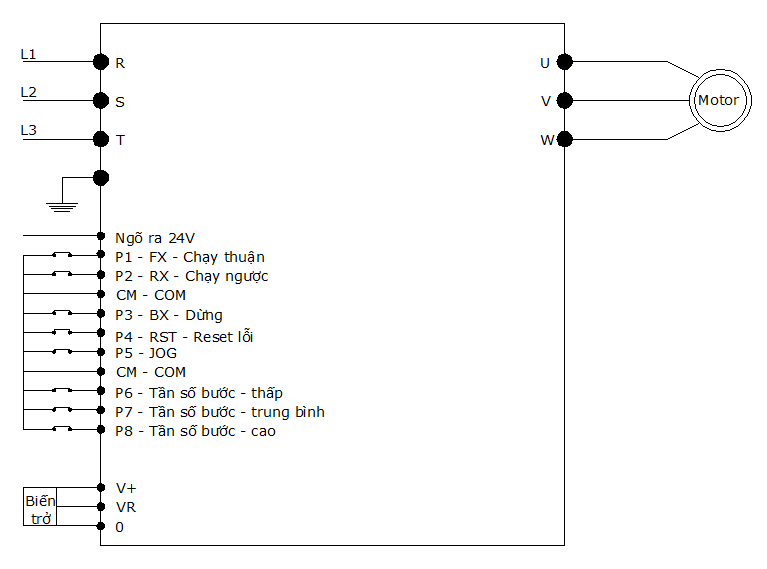
\includegraphics[scale=.7]{1}
\end{center}
\caption{Sơ đồ đấu dây cho các tiếp điểm cần dùng}
\end{figure}
\subsection{Các phím điều khiển}
Gồm các phím sau:
\begin{list}{--}{}
\item Phím Run: Lệnh chạy.
\item Phím STOP/RESET: Dừng khi đang hoạt động và Reset khi có lỗi.
\item Các phím di chuyển: left, right, up, down, dùng để lựa chọn nhóm lệnh, hiệu chỉnh giá trị.
\item Phím xác nhận: Enter (phím giữa), chọn chế độ lệnh để tiến hành cài đặt; lưu giá trị cài đặt vào bộ nhớ.
\item[$\ast$] Chú ý quan sát mã lệnh trên màn hình của biến tần.
\end{list}
\subsection{Các nhóm lệnh điều khiển}
Gồm có 4 nhóm lệnh chính:
\begin{list}{--}{}
\item Nhóm lệnh điều khiển: các lệnh cài đặt thông số biến tần.
\item Nhóm lệnh chức năng 1: Các lệnh hiệu chỉnh điện áp và tần số ngõ ra.
\item Nhóm lệnh chức năng 2: Các lệnh nâng cao, như điều khiển PID.
\item Nhóm I/O: Các lệnh thiết lập tạo trình tự sử dụng các chân đa chức năng.
\end{list} 
\begin{figure}[!h]
\begin{center}
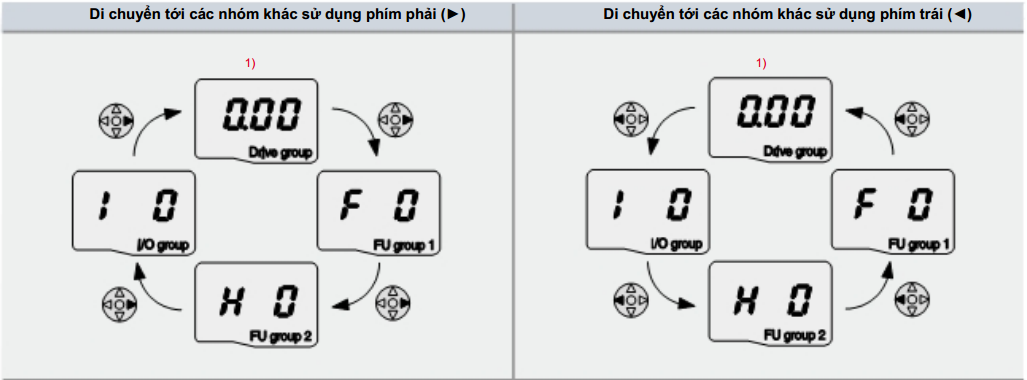
\includegraphics[scale=.5]{2}
\end{center}
\caption{Di chuyển qua lại giữa các nhóm lệnh chính}
\label{Fig:move-cmline}
\end{figure}
Sử dụng các phím Left hoặc Right để di chuyển qua lại giữa các nhóm lệnh chính như hình \ref{Fig:move-cmline}. Nhấn phím Enter (phím giữa) để chọn vào 1 trong 4 nhóm lệnh để cài đặt thông số.
\subsection{Các lệnh cơ bản trong nhóm lệnh điều khiển}
Nhóm lệnh điều khiển bắt đầu bằng ký hiệu \verb|0.00|, kế tiếp là các lệnh:
\begin{list}{--}{}
\item Lệnh \verb|ACC|: Thời gian tăng tốc $t = 0 \div 6000s$.
\item Lệnh \verb|dEC|: Thời gian giảm tốc $t = 0 \div 6000s$.
\item Lệnh \verb|drv|: Chọn chế độ điều khiển. 
\begin{list}{+}{}
\begin{multicols}{2}
\item Chọn \verb|0|: dùng phím.
\item Chọn \verb|1|: dùng \verb|FX/RX-1|.
\item Chọn \verb|2|: dùng \verb|FX/RX-2|.
\item Chọn \verb|3|: dùng \verb|RS-485|.
\end{multicols}
\end{list}
\item Lệnh \verb|Frq|: Phương pháp cài đặt tần số.
\begin{list}{+}{}
\begin{multicols}{2}
\item Chọn \verb|0|: dùng phím -- 1.
\item Chọn \verb|1|: dùng phím -- 2.
\item Chọn \verb|2|: dùng áp $-10V \div +10V$
\item Chọn \verb|3|: dùng áp $0V \div +10V$
\item Chọn \verb|4|: dùng dòng $0V \div +20mA$
\item Chọn \verb|5|: dùng $V1S+1$
\item Chọn \verb|6|: dùng $V1S+I$
\item Chọn \verb|7|: dùng \verb|RS-485|
\end{multicols}
\end{list}
\item Lệnh \verb|st1, st2, st3|: Tần số đặt trước, $f = 0 \div 400Hz$.
\item Lệnh \verb|CUr|: Dòng điện đầu ra $(A)$.
\item Lệnh \verb|rPM|: Tốc độ động cơ $(rpm)$.
\item \ldots
\item Lệnh \verb|drC|: Chọn chiều quay, hiển thị \verb|F| (quay thuận) và \verb|R| (quay nghịch).
\end{list}
\subsection{Các lệnh cơ bản trong nhóm lệnh chức năng 1}
Nhóm chức năng 1 có nhiểu lệnh từ \verb|F0 - F4|,  \verb|F8 - F14|, \verb|F20-F38, F40| và \verb|F50 - F60| trong phạm vi thực hành, quan tâm đến một số lệnh sau:
\begin{list}{}{}
\item Lệnh \verb|F1|: Bỏ chạy thuận/nghịch.
\begin{list}{+}{}
\begin{multicols}{2}
\item Chọn \verb|0|: Chạy thuận/nghịch.
\item Chọn \verb|1|: Bỏ chạy thuận.
\item Chọn \verb|2|: Bỏ chạy nghịch.
\end{multicols}
\end{list}
\item Lệnh \verb|F4|: Chọn chế độ dừng.
\begin{list}{+}{}
\begin{multicols}{2}
\item Chọn \verb|0|: Giảm tốc.
\item Chọn \verb|1|: Hãm DC.
\item Chọn \verb|2|: Tự do.
\end{multicols}
\end{list}
\item Lệnh \verb|F8|: Tần số khởi động hãm DC, $f = 0 - 60Hz$.
\item Lệnh \verb|F9|: Thời gian chờ hãm DC, $f = 0 - 60s$.
\item Lệnh \verb|F10|: Điện áp hãm DC, $0 - 200\%$.
\item Lệnh \verb|F11|: Thời gian hãm DC, $f = 0 - 60s$.
\item Lệnh \verb|F12|: Điện áp khởi động hãm DC, $0 - 200\%$.
\item Lệnh \verb|F13|: Thời gian khởi động hãm DC, $0 - 60s$.
\item Lệnh \verb|F21|: Tần số lớn nhất.
\item Lệnh \verb|F23|: Tần số khởi động.
\item Lệnh \verb|F28|: Bù momen chạy thuận.
\item Lệnh \verb|F29|: Bù momen chạy nghịch.
\item Lệnh \verb|F59|: Lựa chọn chế độ bảo vệ động cơ.
\begin{list}{+}{}
\begin{multicols}{2}
\item Chọn \verb|0|: Bỏ chế độ bảo vệ động cơ.
\item Chọn \verb|1|: Khi tăng tốc.
\item Chọn \verb|2|: Khi chạy ổn định.
\item Chọn \verb|3|: Khi tăng tốc, chạy ổn định.
\item Chọn \verb|4|: Khi giảm tốc.
\item Chọn \verb|5|: Khi tăng và giảm tốc.
\item Chọn \verb|6|: Khi giảm tốc và chạy ổn định.
\item Chọn \verb|7|: Khi tăng tốc, chạy ổn định và giảm tốc.
\end{multicols}
\end{list}
\end{list}
\subsection{Các lệnh trong nhóm I/O}
Các lệnh từ \verb|I17 - I24|:
\begin{list}{+}{}
\begin{multicols}{2}
\item Chọn \verb|0|: Chạy thuận.
\item Chọn \verb|1|: Chạy nghịch.
\item Chọn \verb|2|: Dừng khẩn khi lỗi
\item Chọn \verb|3|: Reset khi lỗi
\item Chọn \verb|4|: Chạy JOG
\item Chọn \verb|5|: Tần số bước thấp.
\item Chọn \verb|6|: Tần số bước trung bình.
\item Chọn \verb|7|: Tần số bước cao.
\item Chọn \verb|8|: Tăng/giảm tốc mức thấp.
\item Chọn \verb|9|: Tăng/giảm tốc mức trung bình.
\item Chọn \verb|10|: Tăng/giảm tốc mức cao.
\item Chọn \verb|11|: Hãm DC khi dừng.
\item \ldots
\item Chọn \verb|15|: Lệnh tăng tần số lên/xuống.
\item Chọn \verb|16|: Lệnh giảm tần số lên/xuống.
\item \ldots
\item Chọn \verb|24|: Bỏ chức năng tăng giảm tốc.
\end{multicols}
\end{list}
\section{Nội dung thực tập}
\subsection{Vận hành thiết bị trên bàn phím bộ biến tần}
\paragraph{Yêu cầu}Thiết lập giá trị cài đặt và điều khiển động cơ bằng bàn phím.
\paragraph{Các chế độ thiết lập}
\begin{list}{--}{}
\item Thiết lập ở chế độ Drive là \verb|0|.
\item Nhấn phím RUN, động cơ tăng tốc trong quá trình hoạt động.
\item Nhấn phím STOP/RESET, động cơ giảm tốc đến khi dừng hẳn.
\item Điều khiển hướng động cơ bằng mã \verb|drC| thông qua bàn phím.
\item Thiết lập giá trị tần số mong muốn, bắt đầu từ \verb|0.00| đến $f < F21$.
\end{list}
\paragraph{Thực hiện}
\begin{list}{--}{}
\item Kết nối động cơ vào các tiếp điểm $U, V, W$ và cấp nguồn cho biến tần.
\item Thiết lập tần số $f = 60Hz$.
\begin{list}{+}{}
\item Từ giao diện: \verb|0.00|, nhấn \verb|Enter|, nhập giá trị \verb|60.00| (kết hợp các phím mũi tên).
\item Bấm \verb|Enter| để lưu giá trị cài đặt vào bộ nhớ.
\end{list}
\item Vận hành và thiết lập tần số: Cấp nguồn.
\begin{table}[!h]
\begin{center}
\begin{longtable}{|c|p{5cm}|c|p{5cm}|c|} \hline
\textit{Bước} & \centering{Lệnh} & \textit{Mã} & \centering{\textit{Mô tả}} & \textit{Giá trị cài đặt} \\ \hline
1 & Bấm phím UP 3 lần & \verb|drv| & Chọn chế độ điều khiển & \\ \hline
2 & Bấm phím ENT và kết hợp với cái phím mũi tên & \verb|0| & Có 4 chế độ lựa chọn, chọn dùng phím &  \\ \hline
3 & Bấm ENT để lưu lại giá trị và trở lại chức năng \verb|drv| & \verb|drv| & Đã chọn chế độ dùng phím & \verb|0| \\ \hline
4 & Nhấn phím UP đi đến mã \verb|Frq| & \verb|Frq| & Chọn phương pháp cài đặt tần số & \\ \hline
5 & Bấm phím ENT và kết hợp với cái phím mũi tên & \verb|0| & Có 8 chế độ lựa chọn, chọn dùng phím &  \\ \hline
6 & Bấm ENT để lưu lại giá trị và trở lại chức năng \verb|Frq| & \verb|Frq| & Đã chọn chế độ dùng phím & \verb|0| \\ \hline
7 & Bấm phím DOWN 4 lần & \verb|60.00| & Trở về giao diện đầu & \\ \hline
\end{longtable}
\end{center}
\caption{Vận hành động cơ qua thiết lập bằng phím}
\end{table}

Hoàn thành quá trình cài đặt điều khiển qua phím.
\item Nhấn phím RUN để vận hành. Điền số liệu thu được vào bảng:
\begin{longtable}{|c|c|c|c|c|c|c|c|}\hline
STT & \multicolumn{2}{|c|}{Dòng điện $(A)$} & \multicolumn{2}{|c|}{Điện áp $(V)$} & Công suất $(W)$ & \multicolumn{2}{|c|}{Tốc độ $(rpm)$} \\ \cline{2-5} \cline{7-8}
& $I_{in}$ & $I_{out}$ & $V_{in}$ & $V_{out}$  & & $Min$ & $Max$ \\ \hline
&  &  &  &   & &  &  \\ \hline
&  &  &  &   & &  &  \\ \hline
&  &  &  &   & &  &  \\ \hline
\end{longtable}
\item Nhấn phím STOP/RESET quan sát và mô tả hiện thỉ của biến tần, và trạng thái của động cơ.
\end{list}
\subsection{Vận hành thiết bị bằng khối tiếp điểm điều khiển}
\begin{list}{--}{}
\item Kết nối $P1$, $COM$, biến trở.
\item Vận hành và thiết lập tần số: Cấp nguồn.
\begin{table}[!h]
\begin{center}
\begin{longtable}{|c|p{5cm}|c|p{5cm}|c|} \hline
\textit{Bước} & \centering{Lệnh} & \textit{Mã} & \centering{\textit{Mô tả}} & \textit{Giá trị cài đặt} \\ \hline
1 & Bấm phím UP 3 lần & \verb|drv| & Chọn chế độ điều khiển & \\ \hline
2 & Bấm phím ENT và kết hợp với cái phím mũi tên & \verb|1| & Có 4 chế độ lựa chọn, chọn dùng \verb|FX/RX-1| &  \\ \hline
3 & Bấm ENT để lưu lại giá trị và trở lại chức năng \verb|drv| & \verb|drv| & Đã chọn chế độ dùng \verb|FX/RX-1| & \verb|1| \\ \hline
4 & Nhấn phím UP đi đến mã \verb|Frq| & \verb|Frq| & Chọn phương pháp cài đặt tần số & \\ \hline
5 & Bấm phím ENT và kết hợp với cái phím mũi tên & \verb|0| & Có 8 chế độ lựa chọn, chọn dùng áp từ \verb|0 - 10V| &  \\ \hline
6 & Bấm ENT để lưu lại giá trị và trở lại chức năng \verb|Frq| & \verb|Frq| & Đã chọn chế độ dùng \verb|0 - 10V| & \verb|3| \\ \hline
7 & Bấm phím DOWN 4 lần & \verb|0.00| & Trở về giao diện đầu & \\ \hline
\end{longtable}
\end{center}
\caption{Vận hành động cơ qua các tiếp điểm}
\end{table}
\vspace{-.5cm}
\item Nhấn nút FWD, quan sát và mô tả hiện thỉ của biến tần, và trạng thái của động cơ.
\item Tăng vào giảm tóc qua biến trở, ghi nhận lại các số liệu:
\begin{longtable}{|c|c|c|c|c|c|c|c|}\hline
Tần số $(Hz)$ & \multicolumn{2}{|c|}{Dòng điện $(A)$} & \multicolumn{2}{|c|}{Điện áp $(V)$} & Công suất $(W)$ & \multicolumn{2}{|c|}{Tốc độ $(rpm)$} \\ \cline{2-5} \cline{7-8}
& $I_{in}$ & $I_{out}$ & $V_{in}$ & $V_{out}$  & & $Min$ & $Max$ \\ \hline
5 &  &  &  &   & &  &  \\ \hline
10 &  &  &  &   & &  &  \\ \hline
15 &  &  &  &   & &  &  \\ \hline
20 &  &  &  &   & &  &  \\ \hline
25 &  &  &  &   & &  &  \\ \hline
30 &  &  &  &   & &  &  \\ \hline
35 &  &  &  &   & &  &  \\ \hline
40 &  &  &  &   & &  &  \\ \hline
45 &  &  &  &   & &  &  \\ \hline
50 &  &  &  &   & &  &  \\ \hline
55 &  &  &  &   & &  &  \\ \hline
60 &  &  &  &   & &  &  \\ \hline
\end{longtable}
\item Vẽ đồ thị: $N = F(f), U = F(f); I = F(f), P = U(f)$.
\item Chỉnh biến trở về vị trí nhỏ nhất và dừng động cơ (nhấn nút \verb|STOP/RESET|.
\end{list}
\subsection{Thiết lập các chế độ vận hành bộ biến tần}
\subsubsection{Thời gian tăng tốc và thời gian giảm tốc của động cơ}
\paragraph{Sơ đồ}Kết nối $P1$, $COM$, biến trở.
\paragraph{Yêu cầu}Thiết lập thời gian tăng tốc trong $10s$ và thời gian giảm tốc trong $10s$.
\paragraph{Cách cài đặt}
\begin{list}{--}{}
\item Bật nguồn cho biến tần.
\item Tiến hành cài đặt theo các bước như trong bảng \ref{Tab:acc}.
\begin{table}[!h]
\begin{center}
\begin{longtable}{|c|p{5cm}|c|p{5cm}|c|} \hline
\textit{Bước} & \centering{Lệnh} & \textit{Mã} & \centering{\textit{Mô tả}} & \textit{Giá trị cài đặt} \\ \hline
1 & Bấm phím UP 1 lần & \verb|ACC| & Chọn cài đặt thời gian tăng tốc & \\ \hline
2 & Bấm phím ENT &  & Chọn để tiến hành cài đặt &  \\ \hline
3 & Dùng phím mũi tên kết hợp với nhập số \verb|10.0| & \verb|10.00| & Thời gian tăng tốc & \verb|10.00| \\ \hline
4 & Bấm phím ENT &  & Xác nhận thời gian cài đặt tăng tốc &  \\ \hline
5 & Bấm phím UP 2 lần & \verb|dEC| & Chọn cài đặt thời gian giảm tốc & \\ \hline
5 & Bấm phím ENT &  & Chọn để tiến hành cài đặt &  \\ \hline
6 & Dùng phím mũi tên kết hợp với nhập số \verb|10.0| & \verb|10.00| & Thời gian giảm tốc & \verb|10.00| \\ \hline
7 & Bấm phím ENT &  & Xác nhận thời gian cài đặt giảm tốc &  \\ \hline
\end{longtable}
\end{center}
\caption{Thiết lập thời gian tăng tốc và giảm tốc}
\label{Tab:acc}
\end{table}
\item Nhấn phím \verb|FWD| (quay thuận) và thay đổi giá trị biến trở, quan sát hiện tượng.
\begin{list}{+}{}
\item Tăng giá trị biến trở:
\item Giảm giá trị biến trở:
\end{list}
\item Chỉnh biến trở về vị trí nhỏ nhất và dừng động cơ (nhấn nút \verb|STOP/RESET|.
\end{list}
\subsubsection{Thiết lặp chạy động cơ trên các ngõ điều khiển}
\paragraph{Sơ đồ}Kết nối $P1,P2$, $COM$, biến trở.
\paragraph{Cách cài đặt}
\begin{list}{--}{}
\item Thiết lập: \verb|drV|: $1$ (qua tiếp điểm).
\item Bấm phím \verb|FWWD|, tăng giá trị biến trở, nhận xét.
\item Nhả phím \verb|FWD|, nhấn \verb|REV|, quan sát hiện tượng.
\item Chỉnh biến trở về giá trị bé nhất. Dừng động cơ bằng cách nhấn nhã \verb|REV|.
\item Thiết lập: \verb|drV|: $1$ (qua tiếp điểm).
\item Bấm phím \verb|FWWD|, tăng giá trị biến trở, nhận xét.
\item Nhả phím \verb|FWD|, nhấn \verb|REV|, quan sát hiện tượng.
\item Chỉnh biến trở về giá trị bé nhất. Dừng động cơ bằng cách nhấn nhã \verb|REV|.
\item So sánh giữa 2 phương án điều khiển trên.
\end{list}
\newpage
\section{Bài tập thực hành thêm}
\subsection{Cài đặt biến tần chạy nhiều cấp tốc độ}
\paragraph{Yêu cầu}Biến tần chạy qua công tắc ngoài (chân $P1$), chạy với 4 cấp tốc độ:
\begin{list}{--}{}
\item Khi vừa khởi động (qua công tắc $P1$): $f_1 = 10Hz$.
\item Bật công tắc $P6$: $f_2 = 30Hz$.
\item Tắt $P_6$, bật công tắc $P7$: $f_3 = 40Hz$.
\item Tắt $P7$, bật công tắc $P8$: $f_4 = 50Hz$.
\item[$\ast$] Tần số cực đại $f_{max} = 50Hz$.
\end{list}
\paragraph{Cách kết nối}Sử dụng $P1$, $P6$, $P7$, $P8$.
\paragraph{Cách cài đặt}
%\begin{table}[!h]
\begin{center}
\begin{longtable}{|c|p{5cm}|c|p{5cm}|c|} \hline
\textit{Bước} & \centering{Lệnh} & \textit{Mã} & \centering{\textit{Mô tả}} & \textit{Giá trị cài đặt} \\ \hline
\multirow{6}{.6cm}{1} & Nhấn phím LEFT 2 lần & \verb|H  0| & Di chuyển đến nhóm chức năng thứ 2 & \\ \cline{2-5}
  & Nhấn phím ENT & \verb|   1| & Chọn nhóm chức năng thứ 2 để cài đặt & \\ \cline{2-5}
  & Kết hợp các phím mũi tên, nhập $40$ & \verb|  40| & Lựa chọn chế độ điều khiển &  \\ \cline{2-5}
  & Nhấn ENT 2 lần & & Chọn lựa chọn chế độ điều khiển để cài đặt & \\ \cline{2-5}
  & Kết hợp các phím mũi tên, nhập $0$ & \verb|   0| & Điều khiển $V/F$ & \\ \hline
  & Nhấn ENT 2 lần & \verb|H 40| & Chọn điều khiển bằng $V/F$ & \verb|H40|, chọn \verb|0| \\ \cline{2-5}
\multirow{2}{.6cm}{2} & Tương tự chọn $H30$ & \verb|H  30| & Lựa chọn công suất động cơ, $kW$ &  \\ \cline{2-5}     
  & Kết hợp các phím mũi tên, nhập $0.75$ & \verb| 0.75| & Công suất động cơ $P = 0.75kW$ &  \verb|H30|, nhập \verb|0.75| \\ \hline     
\multirow{2}{.6cm}{3} & Tương tự chọn $H31$ & \verb|H  31| & Lựa chọn số cưc động cơ &  \\ \cline{2-5}   
  & Kết hợp các phím mũi tên, nhập $4$ & \verb|   4| & Động cơ có 4 cực &  \verb|H31|, nhập \verb|4| \\ \hline     
\multirow{2}{.6cm}{4} & Tương tự chọn $H33$ & \verb|H  33| & Lựa chọn dòng định mức động cơ &  \\ \cline{2-5}     
  & Kết hợp các phím mũi tên, nhập vào giá trị $1.8$ & \verb|  1.8| & Dòng định mức động cơ $1.8A$&  \verb|H33|, nhập \verb|1.8| \\ \hline
\multirow{2}{.6cm}{5} & Tương tự chọn $H34$ & \verb|H  34| & Lựa chọn dòng không tải động cơ &  \\ \cline{2-5}     
  & Kết hợp các phím mũi tên, nhập vào giá trị $0.9$ & \verb|  0.9| & Dòng không tải động cơ $I_0 = 50\%I_{\text{\textit{đm}}}$ &  \verb|H34|, nhập \verb|0.9| \\ \hline
\multirow{3}{.6cm}{6} & Chuyển sang nhóm lệnh điều khiển & \verb| 0.00| &  &  \\ \cline{2-5}     
  & Kết hợp các phím mũi tên, nhập vào giá trị $10$ & \verb| 10.0| & Bật công tắc bắt đầu chạy với $f_1 = 10Hz$ & Nhập \verb|10.0| \\ \cline{2-5}
  & Tương tự chọn $drv$, chọn 1 & \verb| drv| & Chọn điều khiển qua Terminal &  \verb|drv|, chọn \verb|1|\\ \hline     
\multirow{2}{.6cm}{7} & Tương tự chọn $st1$ & \verb| st1| & Cấp độ ở mức thấp &  \\ \cline{2-5}   
  & Kết hợp các phím mũi tên, nhập vào giá trị $30$ & \verb| 30.0| & Cấp độ 2 $f_2 = 30Hz$ (công tắc $P6$) &  \verb|st1|, nhập \verb|30| \\ \hline
\multirow{2}{.6cm}{8} & Tương tự chọn $st2$ & \verb| st2| & Cấp độ ở mức trung bình &  \\ \cline{2-5}   
  & Kết hợp các phím mũi tên, nhập vào giá trị $40$ & \verb| 40.0| & Cấp độ 3 $f_3 = 40Hz$ (công tắc $P7$) &  \verb|st2|, nhập \verb|40| \\ \hline
\multirow{2}{.6cm}{9} & Tương tự chọn $st3$ & \verb| st3| & Cấp độ ở mức cao &  \\ \cline{2-5}    
  & Kết hợp các phím mũi tên, nhập vào giá trị $50$ & \verb| 50.0| & Cấp độ 4 $f_4 = 50Hz$ (công tắc $P8$) &  \verb|st3|, nhập \verb|50| \\ \hline
\multirow{2}{.6cm}{10} & Chuyển sang nhóm lệnh chức năng 1 & \verb|F  0| &  &  \\ \cline{2-5}    
  & Tương tự chọn $F21$, nhập $50$ & \verb|F  21| & Nhập tần số cực đại $f = 50z$ &  \verb|F21|, nhập \verb|50|\\ \hline     
\end{longtable}
\end{center}
%\caption{Cài đặt biến tần chạy nhiều cấp tốc độ qua bàn phím}
%\label{Tab:acc}
%\end{table}
\paragraph{Chạy biến tần}
\begin{list}{--}{}
\item Bật công tắc $P1$, tần số $f_1 = 10Hz$.
\item Bật công tắc $P6$, tần số $f_2 = 30Hz$.
\item Tắt công tắc $P6$, bật công tắc $P7$, tần số $f_3 = 40Hz$.
\item Tắt công tắc $P7$, bật công tắc $P8$, tần số $f_4 = 50Hz$.
\item Tắt công tắc $P1$ để dừng biến tần.
\end{list}
\newpage
\subsection{Cài đặt biến tần để tăng moment xoắn}
\paragraph{Yêu cầu}Lựa chọn bù moment tự động cho động cơ.
\paragraph{Chú ý}Công suất của động cơ và công suất của biến tần phải bằng nhau thì mới bù được (bù tự động hoặc bù bằng tay).
\paragraph{Cách kết nối}Sử dụng $P1$ để chạy biến tần.
\paragraph{Cách cài đặt}
%\begin{table}[!h]
\begin{center}
\begin{longtable}{|c|p{5cm}|c|p{5cm}|c|} \hline
\textit{Bước} & \centering{Lệnh} & \textit{Mã} & \centering{\textit{Mô tả}} & \textit{Giá trị cài đặt} \\ \hline
\multirow{6}{.6cm}{1} & Nhấn phím LEFT 2 lần & \verb|H  0| & Di chuyển đến nhóm chức năng thứ 2 & \\ \cline{2-5}
  & Nhấn phím ENT & \verb|   1| & Chọn nhóm chức năng thứ 2 để cài đặt & \\ \cline{2-5}
  & Kết hợp các phím mũi tên, nhập $40$ & \verb|  40| & Lựa chọn chế độ điều khiển &  \\ \cline{2-5}
  & Nhấn ENT 2 lần & & Chọn lựa chọn chế độ điều khiển để cài đặt & \\ \cline{2-5}
  & Kết hợp các phím mũi tên, nhập $0$ & \verb|   0| & Điều khiển $V/F$ & \\ \hline
  & Nhấn ENT 2 lần & \verb|H 40| & Chọn điều khiển bằng $V/F$ & \verb|H40|, chọn \verb|0| \\ \cline{2-5}
\multirow{2}{.6cm}{2} & Tương tự chọn $H30$ & \verb|H  30| & Lựa chọn công suất động cơ, $kW$ &  \\ \cline{2-5}     
  & Kết hợp các phím mũi tên, nhập $0.75$ & \verb| 0.75| & Công suất động cơ $P = 0.75kW$ &  \verb|H30|, nhập \verb|0.75| \\ \hline     
\multirow{2}{.6cm}{3} & Tương tự chọn $H31$ & \verb|H  31| & Lựa chọn số cưc động cơ &  \\ \cline{2-5}   
  & Kết hợp các phím mũi tên, nhập $4$ & \verb|   4| & Động cơ có 4 cực &  \verb|H31|, nhập \verb|4| \\ \hline     
\multirow{2}{.6cm}{4} & Tương tự chọn $H33$ & \verb|H  33| & Lựa chọn dòng định mức động cơ &  \\ \cline{2-5}     
  & Kết hợp các phím mũi tên, nhập vào giá trị $1.8$ & \verb|  1.8| & Dòng định mức động cơ &  \verb|H33|, nhập \verb|1.8| \\ \hline
\multirow{2}{.6cm}{5} & Tương tự chọn $H34$ & \verb|H  34| & Lựa chọn dòng không tải động cơ &  \\ \cline{2-5}     
  & Kết hợp các phím mũi tên, nhập vào giá trị $0.9$ & \verb|  0.9| & Dòng không tải động cơ $I_0 = 50\%I_{\text{\textit{đm}}}$ &  \verb|H34|, nhập \verb|0.9| \\ \hline
\multirow{3}{.6cm}{6} & Chuyển sang nhóm lệnh điều khiển & \verb| 0.00| &  &  \\ \cline{2-5}     
  & Kết hợp các phím mũi tên, nhập vào giá trị $50$ & \verb| 50.0| & Bật công tắc bắt đầu chạy với $f5 = 10Hz$ & Nhập \verb|50.0| \\ \cline{2-5}
  & Tương tự chọn $drv$, chọn 1 & \verb| drv| & Chọn điều khiển qua Terminal &  \verb|drv|, chọn \verb|1|\\ \hline     
\multirow{2}{.6cm}{7} & Chuyển sang nhóm lệnh chức năng 1 & \verb|F  0| &  &  \\ \cline{2-5}    
  & Tương tự chọn $F21$, nhập $50$ & \verb|F  21| & Nhập tần số cực đại $f = 50z$ &  \verb|F21|, nhập \verb|50|\\ \hline  
\multirow{2}{.6cm}{8} & Tương tự  chọn $F27$& \verb|F 27| & Lựa chọn phương pháp bù moment&  \\ \cline{2-5}    
  & Kết hợp các phím mũi tên, chọn 1 & \verb|   1| & Bù tự động &\verb|F27| chọn \verb|1| \\ \hline 
\end{longtable}
\end{center}

Ở \textit{bước 8}, nếu chọn bù bằng tay (chọn \verb|F27| rồi chọn \verb|0|) thì tiếp tục cài đặt \verb|F28| và \verb|F29| là bù moment khi chạy thuận và bù moment khi chạy ngược).
\paragraph{Chạy biến tần}
\begin{list}{--}{}
\item Bật công tắc $P1$, tần số $f = 50Hz$.
\item Tắt công tắc $P1$ để dừng biến tần.
\end{list}
\end{document}